\documentclass[12pt,a4paper]{article}
\usepackage{tikz}
\usepackage{graphicx}
\usepackage{hyperref}
\usepackage{verbatim}
\usepackage[font=small,labelfont=bf]{caption}
\usepackage{geometry}
%\geometry{showframe=true}
\geometry{a4paper,margin=1.25in}

\usepackage[right]{lineno}
%\nolinenumbers
\linenumbers
\modulolinenumbers[5]

\usepackage{amsmath}
\usepackage{caption,float}
\usepackage{icomma}
\captionsetup[table]{skip=8pt}
\newcommand{\millper}{ &\multicolumn{3}{c}{\textsc{aud millions}}
  &\multicolumn{3}{c}{\textsc{percentages}}\\}

\newcommand{\labper}{ &\multicolumn{3}{l}{\textsc{fte employees}}&
  \multicolumn{3}{r}{\textsc{percentages}}\\}

\newtheorem{remark}{Remark}

\title{Boyne Smelters and Gladstone Power Station\\\vskip5pt
  \large{Economic Impact on the
  Gladstone Region and Queensland}}
\author{\small Patrick O’Callaghan and John Mangan}
\renewcommand\thefigure{(\roman{figure})}
\begin{document}

\maketitle

\section*{\centering Outline}


In this study, we consider the economic impact of shutting down Boyne Smelter
Limited (BSL) and the Gladstone Power Station (GPS). To disentangle the
effects of each closure, we study two main scenarios: the one where only the
smelter closes; and the one where both the smelter and the power station
close. To ensure our conclusions are robust, we study different subscenarios
that capture various economic response by key agents in the economy. For
instance, in one subscenario, local refiners of Aluminium Oxide (AlOx) that
supply BSL are able to increase exports in response to the closure of BSL, so
that their revenue is unaffected. By implicitly allowing our economic agents to
respond and, implicitly allowing prices to move, our analysis goes well beyond a
basic multiplier analysis.

The Gladstone region is home to both BSL and GPS. For this reason the Gladstone
region (Statistical Area Level 3, SA3) is at the center of our model. Yet the
closure of BSL and GPS would have potentially significant repercussions outside
of Gladstone, both upstream (Bauxite (Bx)) and downstream (fabrication of
aluminium products, vehicle manufacturing as well as the National Electricity
Market (NEM) itself). In our analysis of economic inputs and outputs, we
therefore include some relevant transactions from the wider Queensland economic
network. In particular those that relate to aluminium. Although we do model
scenarios where GPS remains open and supplies various amounts of electricity to
the grid, and we do so with implicit movements in electricity prices in mind, a
key exclusion from our analysis is the likely broader impact on electricity
prices of the closure of BSL or GPS on the National Electricity Market.

Whilst the broader effect of a BSL closure on Queensland electricity prices is
likely to be welfare increasing, the immediate downside would be 920 direct job
losses in the Gladstone region. Based on US estimates, high-level research by
QTC suggests that total job losses (direct plus indirect effects), might be as
high as 3,000: that is 10\% of the SA3 Gladstone workforce.

Our analysis suggests that job losses would only be reach this figure in the
scenario where both BSL and GPS were closed or in the worst-case scenario where
exports fail to absorb key transactions in AlOx and Electricity. If only the
smelter were to close, then the most likely outcome would be somewhere in the
vicinity of 2000 total job losses. If both the smelter and the power station
were to close, then total job losses would indeed be in the vicinity of 3500. 
Both of these estimates are for a broader definition of Gladstone than SA3, as discussed above. 

We arrive at these figures through \emph{extraction analysis}. This involves
removing all the purchases (inputs) and all the sales (outputs) associated with
BSL from the local economy. This extraction of BSL goes beyond a shock
to final demand: every link that connects BSL to the rest of the economy is
deleted. In the likely intermediate-case scenarios, exports almost fully replace
the key transactions in AlOx and Electricity and BSL sales to downstream sectors
are almost fully replaced by imports of aluminium.  For GPS, given that it
employs approximately one third of the total employees of the Electricity Supply
sector, we extract one third of the latter sector. Though we also fully extract
a key purchase of thermal coal.

The magnitude of the subsidy to BSL (via CS Energy and electricity prices) is significant. An important proviso is that the present study does not account for any change in government spending other than the removal of this subsidy. What we do find is that our results are sensitive to proportion of the subsidy that we treat as endogenous to the economy. We assume \$40\textsc{m} of the subsidy is endogenous to the economy and part of Gross Value Added. The removal of this subsidy to BSL amounts to an increase in GVA has knock-on effects via the public sector multiplier. If half or more of this subsidy is treated as endogenous, its removal swamps the negative effects of the closures. If the endogenous portion of the subsidy significantly smaller than \$40\textsc{m}, then the effect is to magnify the multpliers. These findings are robust to whether the subsidy enters via the Aluminium or Electricity sectors. We take this to mean that there is a significant role for public policy in the transition of the Gladstone economy. 

In summary, the key output of the current work is to provide a working model of the broader Gladstone economy. This model is built on the basis of the latest input-output tables from the Australian Bureau of Statistics, Gladstone regional data and a careful reconstruction of the following cost functions: BSL; the two Gladstone Alumina refineries QAL and Yarwun;  and GPS. We run various scenarios through model to study and estimate the likely impact of the shutdown of BSL and GPS.

\section*{\centering Aluminium smelting in Australia}
 
Although Australia is the 5th largest producer of Aluminium in the world, Australia’s
aluminium smelting industry is in long-term decline. In part, this is due to
increased global supply of (unwrought) aluminium, but it is also because
Australia has lost one of its comparative advantages: low energy prices. This loss
is a consequence of two key underlying countervailing forces in electricity markets
\begin{itemize}
\item the deregulation of the Australian electricity market that began in 1998
\item the absence of investment in new and genuinely cheap sources of energy.
\end{itemize}
Cheap energy is the basis of a thriving manufacturing industry and deregulation
made it harder to justify subsidies to smelters. Over the last two decades, market prices for electricity
have pushed Australian smelters from the top quartile to the bottom quartile in
terms of international competitiveness.

\subsection*{ \centering Smelter closures}

These conditions have already led to
the closure of two smelters: Kurri-Kurri in 2012 and Point Henry in 2014.  In
addition to Boyne Island, there are now three other remaining smelters in
Australia: Bell Bay, Tasmania; Portland, Victoria; and Tomago, NSW. In the last
six months the potential closure of the Portland smelter has been in the news. 

Between 2014 and 2019, factors such as a weaker Australian dollar and
restrictions on winter production in China have provided smelters with a
short-to-medium term buffer. But, even before the recent coronavirus outbreak,
global aluminium prices were around \textsc{usd}1,800 and close to the short-run
minimum average cost of producing aluminium for BSL.

\subsection*{\centering Boyne Island vs Tomago}

BSL accounts for $25\%$ of Australian annual production of Aluminium.  Tomago is
very similar to BSL in terms of size, age, salary and other input costs, and it
is also majority owned by RT. In contrast with Tomago, BSL produces
significantly below its annual capacity of $584$\textsc{kt}. In each of 2017,
2018 and 2019, BSL produced $500\textsc{kt}$ . Under the Interconnection and
Power Pooling Agreement (IPPA), BSL is allocated $810\textsc{mw}$ (per hour) of GPS output.
 At $500\textsc{kt}$ per annum, the implied quantity of
electricity consumed is $798\textsc{mw}$ (per hour). Since BSL has restricted its output to the base load supply, thereby avoiding electricity purchases at wholesale prices (see \cite[slide 10]{Brook} for further details
 of events that lead to this situation). 


Our recommendation is that, before deciding the joint future of BSL and GPS, the
QLD government should have a clear understanding of the subsidy that NSW
provides the Tomago smelter. The subsidy seems to be the only plausible
explanation for the difference in output between BSL and Tomago.

\subsection*{ \centering Subsidies}\label{sec-subsidy}

Subsidies to aluminium smelting have been well-debated in Australia for over 20
years \cite{subsidies}. In 2015, the Government-Owned Corporation CS Energy  
described its contractual obligation to GPS as onerous \cite[page 10]{CSE}.

In our calculations, we assume that BSL pays around $\$55$
per \textsc{mwh}. This is significantly lower than the Queensland wholesale
prices of around \$80 in 2019. Assuming that BSL would pay wholesale prices in
the absence of a subsidy, we estimate that the subsidy per \textsc{mwh} to
aluminium production at BSL is $\$25 $.  Using the fact that $14\textsc{mwh}$
are required to produce a single tonne of aluminium, and BSL produces
$499 \textsc{kt}$, given this data, we are able to obtain a precise estimate of
the subsidy to aluminium production at BSL, approximately
\[\$ 174.65\textsc{m} = \$25 \cdot 14 \cdot 499\textsc{k} \] 
We note that even
if the subsidy is only \$20 per \textsc{mwh}, it does not significantly affect
our results. 
Nor does it matter whether we model this key purchase of $6,986\textsc{gwh}$ of Electricity net of the subsidy or gross:
\[\$ 558.8\textsc{m} =\$80 \cdot 14 \cdot 499\textsc{k}. \] 
\begin{figure}[ht]
  \caption{  \label{fig-Bx-ratio} The structure of the Interconnection and Power Pooling Agreement}
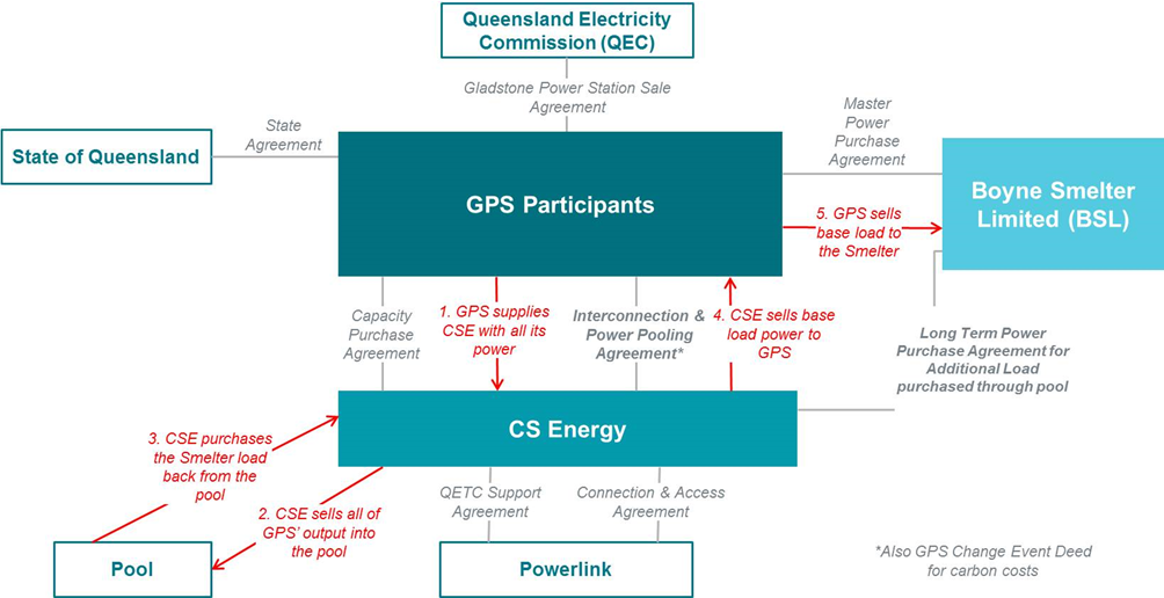
\includegraphics[width=0.98\textwidth]{./ippa.png}
\vskip5pt
   \caption*{\footnotesize 
   CSE sells GPS's Electricity output at wholesale prices (\$80) and sells the base load quantity of approximately $7,000\textsc{gwh}$ per annum back to BSL (indirectly via GPS) at prices net of subsidy (\$55). This has lead it to publicly describe its contract with GPS as onerous.}
  \end{figure} 
What does matter is the extent to which the subsidy is endogenous to the economy (see discussion below). This sensitivity is a result of the public-sector multiplier,  suggesting that, if enough of the subsidy were to remain in the economy after shut down of BSL, then it would reverse any negative effects.

\subsection*{ \centering Gladstone (and Queensland) aluminium exports}

There has been a marked decline in the diversity of the export market relative
to the period 2000-2010. Since 2014, four countries, all long-term political
allies of Australia, account for almost all the exports of Gladstone
aluminium. In order of magnitude Japan, the Republic of Korea, the US and
Taiwan.  Japan purchases over 200\textsc{ktpa}. The Republic of Korea then
follows with purchases typically ranging between 50 and 100\textsc{ktpa}.

This absence of diversity in Aluminium exports stands in contrast with
Queensland exports in the upstream markets of Alumina and, more recently,
Bauxite.

\subsection*{ \centering Key upstream  markets}
For many years, Gladstone has been an integral part of RT’s vertically
integrated approach to aluminium production in Queensland. From bauxite (Bx)
mining in the Weipa region of Far North Queensland, to alumina (Aluminium Oxide,
AlOx) refinement, electricity (El) generation and aluminium (Al) smelting, all
in the Gladstone region.

At regular intervals during the last decade (2011, 2015 and 2018), RT has
unsuccessfully attempted to sell its Pacific Aluminium portfolio of assets.
With the completion of the commissioning of the \$1.9 billion Amrun bauxite mine
at Weipa in March 2019, RT has established independence of bauxite
production \cite{RT}.  On the demand side, the main driver of the recent increase exports of Weipa Bauxite is
demand from China.

\begin{figure}[ht]
  \caption{  \label{fig-Bx-ratio} Gladstone imports of Bauxite as a proportion
    of Weipa production (Gladstone Port Data)}
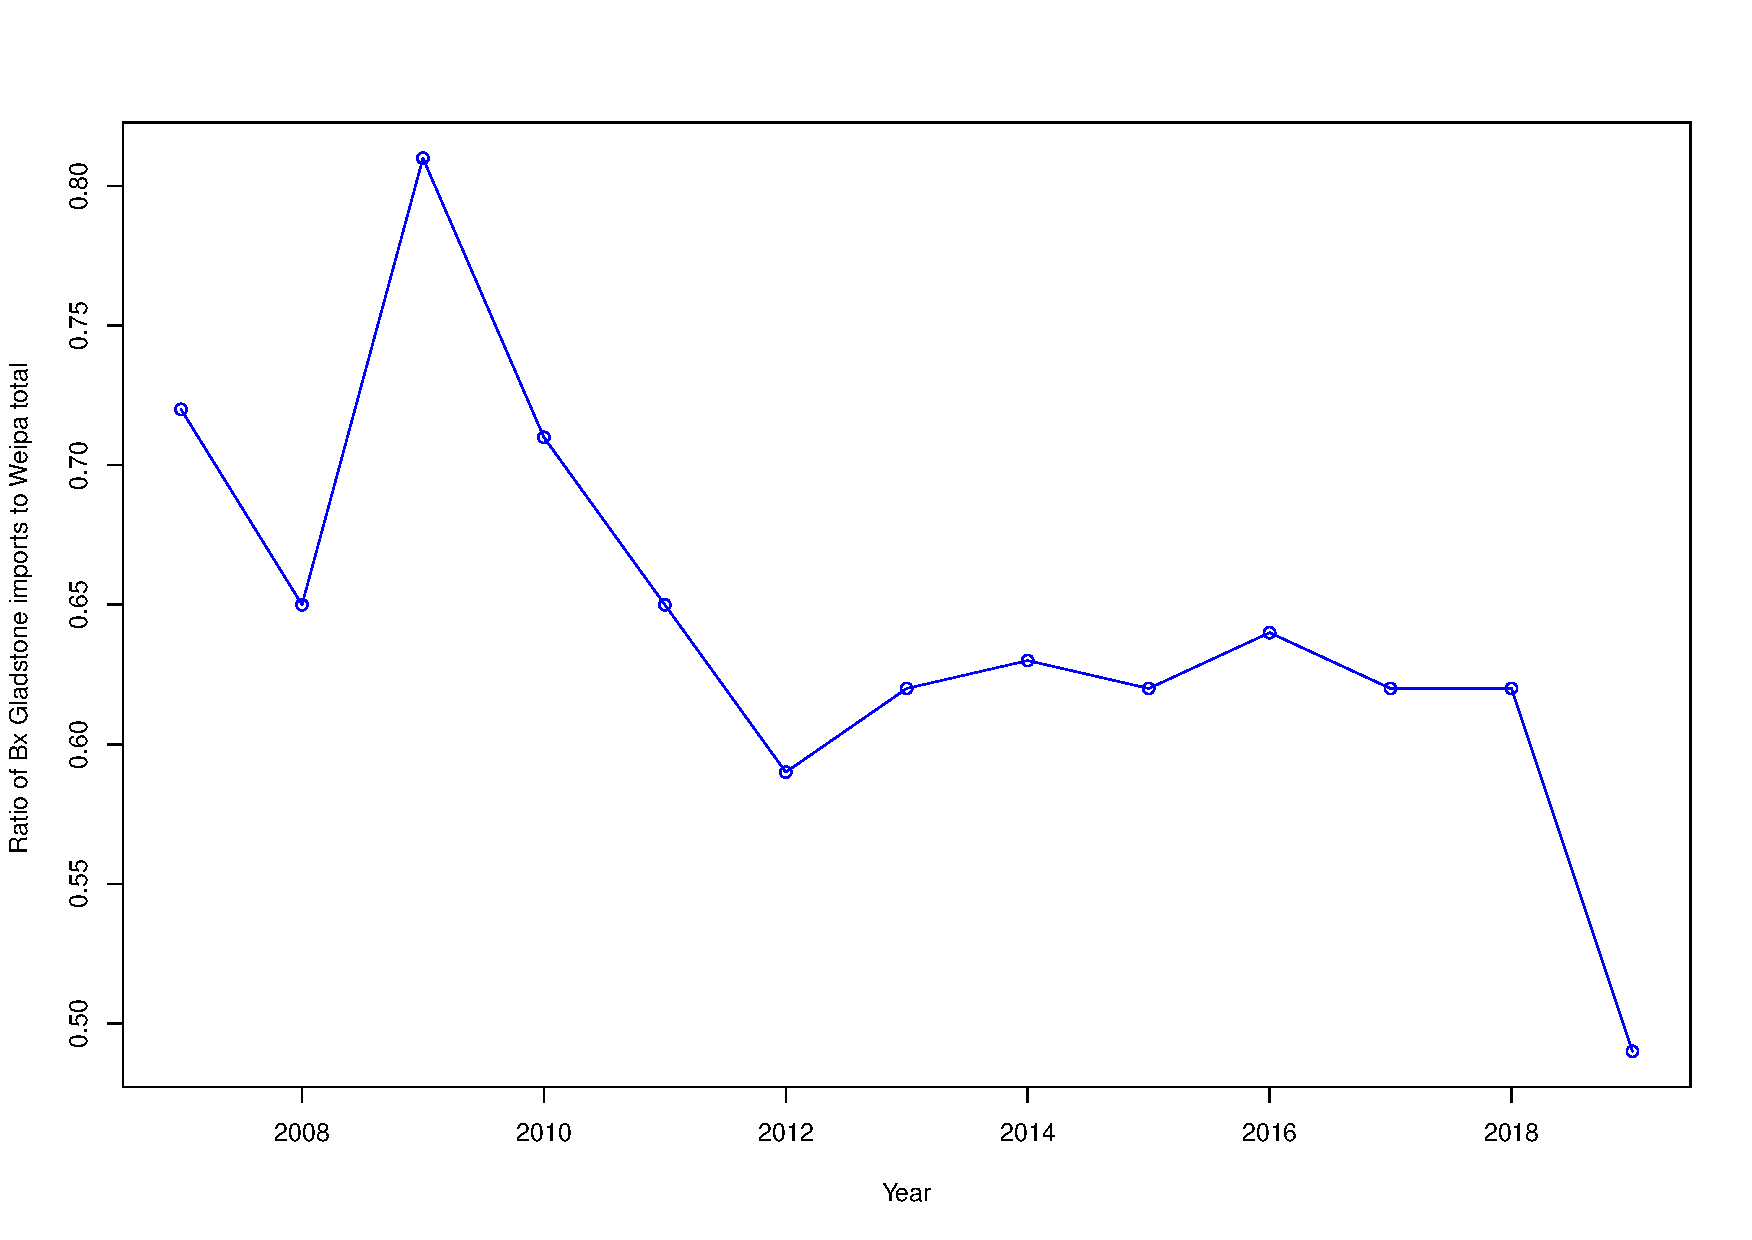
\includegraphics[width=0.98\textwidth]{./Bx-imports-ratio.pdf}
   \caption*{\footnotesize Over time, Weipa Bauxite production has become
    less dependent on Gladstone Alumina refining. Since the Amrun mines opened
    in 2019, less than half of Weipa Bauxite arrives at Gladstone}
  \end{figure} 

  Via Gladstone Port data, in 2019, imports of Bx to Gladstone from Weipa stood
  at 17,397.6\textsc{kt}. According to the RT 2019 Annual Report, this Bx is
  then refined into 6,545\textsc{kt} of AlOx at Gladstones two refineries:
  Queensland Alumina L\textsc{td} and Yarwun Alumina Refineries. (RT owns 80\%
  and 100\% of these respectively.) Of this total Gladstone output of AlOx, 15\%
  (1000 \textsc{kt}) is sold to BSL for smelting into unwrought Al. The rest is
  shipped to a wide range of international destinations.

\begin{figure}[ht]
  \caption{  \label{fig-AlOx-exports} Gladstone exports of Alumina (AlOx) (Gladstone Port Data)}
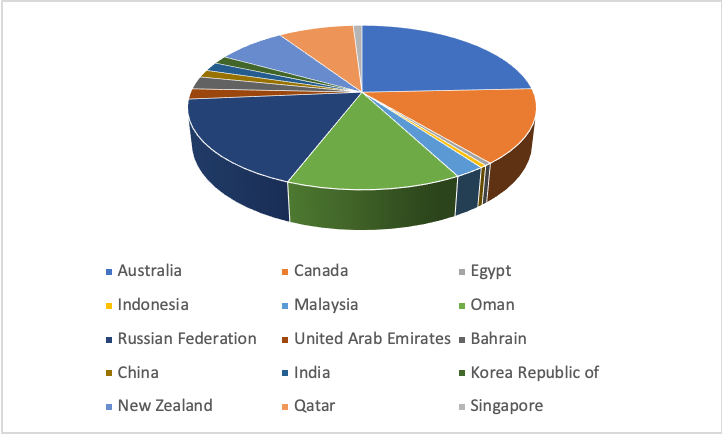
\includegraphics[width=0.98\textwidth]{./fig-AlOx-exports.png}
   \caption*{\footnotesize 
   The diversity of this export market suggests that Alumina refining in Gladstone is largely independent of BSL. (For an interactive version of this chart see the slides.)}
  \end{figure} 

  This diversity of export destinations bodes well for the upstream sector in
  the event of a BSL closure. Yet 15\% is a significant volume of sales, and the
  potential for a small fall in revenues cannot be dismissed. Thus, in the
  intermediate economic scenarios that we model below, we specify a
  50\textsc{kt} fall in quantity sold that is 5\% of the amount of AlOx that BSL
  currently purchases. In other words, just under 1\% of Gladstone total sales
  of AlOx. In the worst case scenarios, partly as a matter of completeness and
  partly in view of the current Covid-19 crisis, we suppose that RT fails to
  replace the BSL purchase, so that Gladstone AlOx sales volumes fall by 15\%.

  Further evidence of the likely resilience of Gladstone AlOx production to a
  BSL closure is the fact that RT recently moved its Alumina and Hydrates
  research facility from Brisbane to Yarwun at Gladstone. The University of
  Queensland participates in that research. In early 2020, mineral
  development company Alpha HPA (High Purity Alumina) announced that it will
  open a $\$200\textsc{m}$ plant in Gladstone with the 
  growing demand from market for batteries in mind.\footnote{www.australianmining.com.au/news/gladstone-welcomes-200m-alumina-plant/}
  This shows that there is a clustering of businesses that are seeking to build
  on the existing expertise in the area.

  
\subsection*{ \centering Local sales of aluminium}
We are able to obtain a coarse picture of the local downstream purchasers of
Aluminium by looking at the difference between international exports (via the
Gladstone port data) and BSL production. On average, over the last 15 years, BSL
production has exceeded international exports by 189\textsc{ktpa}. Assuming
local demand is more-or-less constant, this implies that almost two-fifths of
BSL production is sold to downstream manufacturers in the Gladstone region, and
more broadly in South-East Queensland. The desire to capture the impact on these
sectors as well motivates our slightly broader definition of Gladstone.

Although global prices are unlikely to move as a consequence of a 25\% reduction
in Australian capacity for smelting, local prices for aluminium may well rise as
a consequence of BSL’s closure. It is often the case that smaller industries
cluster around large producers of basic products. As a consequence, we will
include a small knock-on effect on local aluminium prices as one of the economic
scenarios we model.




\section*{ \centering Electricity generation in Gladstone}


At 14\% of existing capacity, GPS is Queensland’s largest
power generator.   It is therefore a key part of Queensland’s coal-fired fleet of
power stations which, altogether, provide three-quarters of existing
supply. Since the closure of Hazelwood (coal-fired) generator of Victoria in
early 2017, Queensland has been a net exporter of electricity to NSW. Eastern
Australia’s dependence on Queensland coal will increase further following the
upgrade to an existing interconnector in late 2021. This upgrade is part of the
Australian government’s broader strategy to secure energy supplies in time for
the closure of the Liddell (coal-fired) power station of NSW in early
2023.

Although GPS will turn fifty in 2026, recent investment in upgrades by GPS operator
NRG (a US firm) ensure that it has the capacity to remain beyond 2029
\cite{GPS-2029}. Indeed, the Draft Integrated System Plan \cite[page 71]{AEMO}
of Australian Energy Market Operator (AEMO) states

\begin{quote}
  “After the closure of Gladstone Power Station (currently expected in 2035),
  network upgrades are required to supply loads in the Gladstone area.”
\end{quote}
\subsection*{\centering A variable-load, coal-fired power station}
Most coal-fired power stations are of base-load type. That is they do not have
the machinery in place to vary output in response to supply and demand shocks.
This is the case for the other coal-fired power stations in Queensland (Kogan
and Callide). In contrast, GPS is a variable-load power station making it
well-suited to accommodating possible intermittencies that  arise due to
renewable energy supply.

In isolation, the immediate closure of BSL would have a significant downward
impact on the price of electricity in Queensland. This impact is measured both
in terms of a reduced average price on the one hand, but increased volatility on
the other. Although BSL consumes approximately half of GPS energy capacity,
because GPS operates well below capacity (between 50\% and 60\% of capacity on
average) the proportion of BSL electricity consumption to GPS output is perhaps
close to 75\%. Whilst this alone would suggest that GPS is entirely dependent on
BSL, GPS in fact supplies the grid in open competition with other suppliers. In
other words, the subsidy flows to BSL, not GPS. The key transaction
BSL\_Electricity is between the grid and BSL, not GPS and BSL.

We conclude this section reiterating that the potential increase in variation in
electricity prices or potential blackouts that might arise if the capacity of
GPS were removed from the East coast grid plays no role in the input-output
analysis of this report. The potential disruption caused by such events (if any), should
be seen as over-and-above the impact that we calculate.



\section*{ \centering The Input--Output Model}

  
\subsection*{ \centering The challenges of “scrubbing” the data}\label{scrubbing}
Perhaps the most challenging task is that of scrubbing the data and building the
appropriate Input–Output table. Our initial table is the latest Australian
Bureau of Statistics (ABS) “Industry by Industry Flow Table (Direct Allocation
of Imports)” for Australia \cite{abs}. One key observation is that this table
subsumes Alumina Refining into Non-ferrous Metal Mining. Since there is no other
mining in Gladstone of this form, we convert this Australian sector into
Gladstone AlOx refining. We also convert Non-ferrous Basic Metal Manufacturing
into the BSL sector for closure.  We then estimate the cost functions for these
two key sectors, on the basis of “hard” micro-level data such as Port of
Gladstone Trade Statistics \cite{port}, Annual Reports (of RT in particular,
\cite{RT}).  We also obtain key output, capacity, possible exports and cost
information concerning GPS with some of the information coming from QTC
including two reports: \cite{Dann} and \cite{Brook}.\footnote{We thank Graham
  Phelan and Liam Ramke for their help in this process.} In contrast with AlOx
and Al production, which are each allocated their own dedicated sectors, we
model a single Electricity Supply with GPS as an important part. We also pulled
in key aspects of upstream and downstream sectors, use Location Quotients based
on Queensland Regional Profiles data \cite{reg-prof} and Gladstone Regional
Council Data \cite{id-comm}.

% \subsection*{ \centering Modelling methodology: extraction}
 
% The IO framework assumes perfect elasticity of supply up to capacity
% constraints. For heavy industry such as aluminium smelting and electricity
% generation, these are reasonable assumptions.

% Beyond aluminium smelting, there
% is the question of upstream impact. Would global markets absorb the resulting
% excess supply of alumina and bauxite, or would the closure of GPS and BSL also
% result in reductions in Queensland output and employment in these markets? To
% allow for an analysis of the impact on welfare that stems from movements in
% electricity prices and the global market prices for alumina and bauxite, we will
% conduct a partial equilibrium analysis using best estimates of supply and demand
% curves. %  Estimation of potential subsidies requires evaluation of welfare and,
% therefore, the specification of a welfare function. We will propose a simple,
% linear, utilitarian form and explain how it can be modified to accommodate and
% evaluate additional preferred pathways. The dollar value of the optimal subsidy
% that the Queensland Government might be willing to pay to avoid closure of BSL
% can be derived from the above analysis. Different social welfare functions will
% of course lead to different dollar values and the ultimate choice therefore lies
% with the Queensland Government.

\subsection*{ \centering Software}
In addition to Excel and Numbers, we use both The R Package (and RStudio in
particular) for Input–Output modelling and the IO8 software to cross-validate
our calculations; and Emacs for producing the report using the Latex mark up
language.

\subsection*{ \centering The Local Economy: Gladstone-plus}
We refer to the local economy of our model as Gladstone-plus. This is the  \emph{SA3
Gladstone region plus key sectors in Queensland that are upstream and downstream
of BSL}. That is, we subsume key parts of the production of upstream Bx
production, and the downstream South-East Queensland sectors for Aluminium
Product Fabrication, Transport Manufacturing and Equipment Manufacturing, in our
definition of “local economy”. For Bx, this inclusion is modelled by adding Bx
imports to the main diagonal of the intermediate production matrix and reducing
imports accordingly. For the downstream sectors, we expand relevant intermediate
transactions and exports for these three sectors.

Once these inclusions have been made the IO table needs to be rebalanced so
that, for each sector $i$, Total Inputs (the vertical sum on an IO table) is
equal to Total Output (the horizontal sum on an IO table).  We do this by
holding the columns for AlOx, Al and El constant whilst calibrating the rest the
table to these parameters in an iterative process that resembles an implicit
form of equibration. This rebalancing process brings the proportions of the
table into line with the original data that we started with: the 2019 release of
the ABS 2016-2017 IO table for Australia (see section \ref{scrubbing} for
details). In particular, Gross Domestic Value Added as a proportion of Total
Output (net of imports) for the Australian table is approximately $33\%$. This
roughly matches our ratio of $31.6\% $. Small differences are inevitable because
of our inclusion of upstream and downstream sectors as part of our effort to
model the impact on the wider Queensland economy.

As per the Australia Table, we define Gross Value Added (GVA) as the sum of
Employee Compensation, Gross Surplus and Tax (minus subsidies) on
Production.\footnote{The sum of P1, P2 and P4 on the Australian IO table.} For Broader Gladstone, this is
\[ \$7,782.5\textsc{m} \approx 3,392 + 3,398.5 + 402.4 \]

In the table that follows, percentages are relative to    
\begin{quote}
Net Local Output = Intermediate Production + GVA.
\end{quote}
For Gladstone-plus, this number is \$13,295.4\textsc{m}, and, for Australia, it is
\$3,060,572\textsc{m}.    
\begin{table}[H]
\centering
\caption{\label{tab-Glad-Aus} Comparison of aggregate figures } 
\begin{tabular}{lrr|rr}
&\multicolumn{2}{r}{Gladstone-plus}& \multicolumn{2}{l}{Australia}\\
  \hline
 & \$ \textsc{m} &  \%&\$\textsc{m}  & \%  \\ 
  \hline
Total Intermed. & 5,669.9 &42.7 &1,416,011& 46.3\\
Employ. Comp. & 3,382.9& 25.4 &833,249& 27.2\\
Gross Surplus & 4,022.6& 30.3 &752,565& 24.6\\
Tax on Prod'n & 220.0& 1.65&  58,747 &1.9\\
  Gross Value Added &7625.5 & 57.4 & 1,644,561  & 53.7\\
   \hline
\end{tabular}
\end{table}

On aggregate, these proportions for  Gladstone-plus are sufficiently similar
to those of Australia.  Gladstone-plus is 
specialised in manufacturing and, for this reason, Labour’s Share of GVA, at
$44.3\%$, is relatively low compared to regions with  labour-intensive sectors
\cite{manu-lab-share}. The trend towards low Labour shares is a long-term one
 that is currently the subject of intense debate and research the current economics 
 literature.  Since Gladstone
is a relatively small region, the proportion of Imports to Regional  Output is $\$4,225.6\textsc{m}$ ($31.8\%$) is between five and six times higher than that of Australia. This number is actually lower than the NIEIR figure (via economy.id.com) for Gladstone of $\$7,373.4\textsc{m}$ because we have pulled dependent upstream and downstream industries into the economy of Gladstone-plus. If, for instance, we were to treat Bauxite as an import to Gladstone-plus, rather than as part of the internal economy, our imports would rise to approximately $\$5,000\textsc{m}$.

For this extended definition of the Gladstone regional economy, we obtain an
implied or \emph{effective workforce} of approximately 31,700 \textsc{fte} employees. This is
approximately 1,700 higher than QTC estimate of 30,000 in
\cite[page 16]{Dann}.\footnote{This is a 2018 estimate by the National Institute of
  Economic and Industry Research} The Regional Profile figure for 2016 was $26,594$ of which only $17,603$ are full-time.  Our figure therefore includes
contractors and commuters to Gladstone from South East Queensland, as well as
representative component of related upstream and downstream employment. It is
relative to this benchmark that we measure changes in employment in the
scenarios we study.

\subsection*{\centering The Input–Output  matrix of transactions}

In figure \ref{fig-heatAcomp}, we present  part of the
status quo transaction matrix. All scenarios involve modifying this transaction
matrix and then comparing with the status quo.  
\begin{figure}[ht]
  \caption{\label{fig-heatAcomp} The transactions matrix
    (\textsc{aud} millions) for the status
    quo Gladstone-plus economy: sectors 5–34
    and Compensation of Employment }
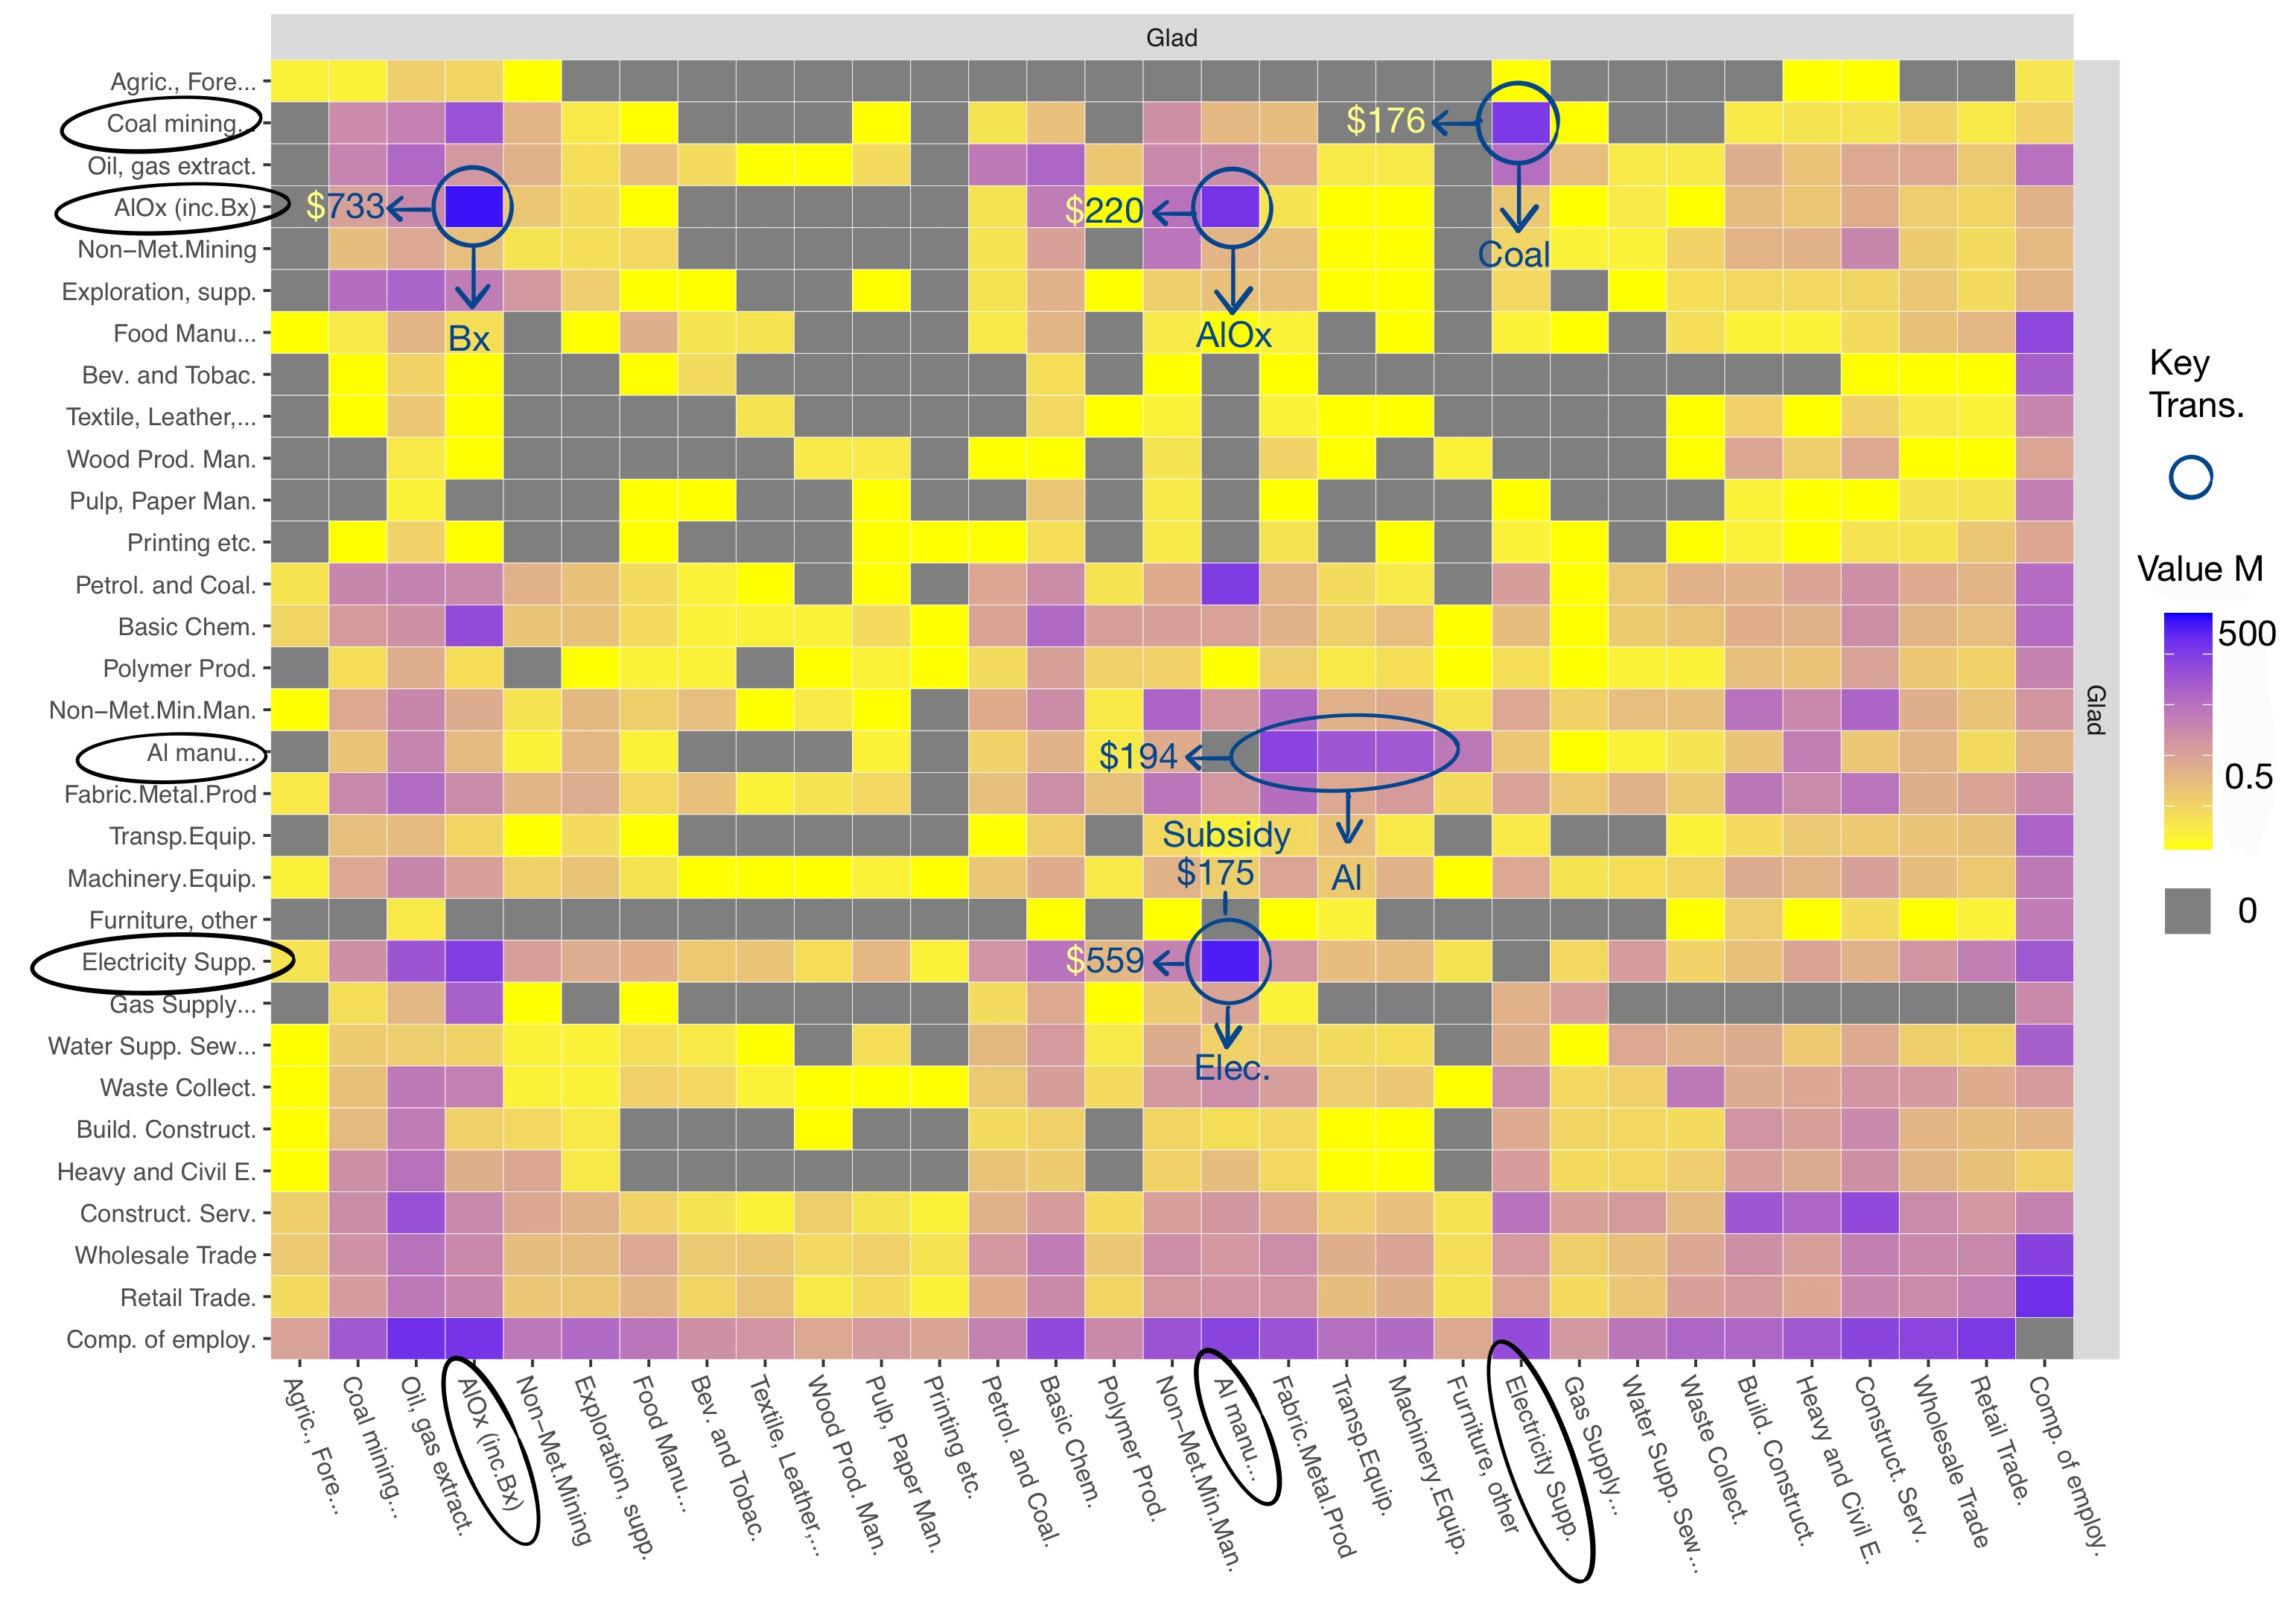
\includegraphics[width=.98\textwidth]{./heatZvalcomp-ann.jpg}
\caption*{  This heatmap provides a visual description of a fragment of the Input–Output table of transactions. Key, large transactions are represented by blue or violet squares. Yellow transactions are smaller. Grey stands for zero/no transaction. When we extract BSL from the economy, we assign a zero to every entry in the row and column indexed by “Al manu...”. (It is the only Basic Nonferrous-Metal Manufacturer in the region.)}
  \end{figure}
\subsection*{\centering The scenarios}

The  two overarching scenarios we consider correspond to the closure
of BSL alone and the joint closure of BSL and GPS. 
\begin{enumerate}
\item\label{Al} Full extraction of BSL from the local economy plus the following  upstream
  and dowstream pricing subscenarios:

  \begin{enumerate}
  \item\label{Al-full} Full replacement of key BSL purchases (of AlOx and El) by exports;
    downstream manufacturing parameters are uneffected.
    
\item\label{Al-par} Partial replacement of key BSL purchases by exports
  (95\% of AlOx and 80\% of El); downstream manufacturing faces 5\%
  extraction;
    
  \item\label{Al-none} Nonreplacement of BSL purchases by exports;
    downstream manufacturing faces 5\% extraction.
     
    \end{enumerate}
  \item\label{AlEl} Full  extraction of BSL  and one-third extraction of
    El from the local economy, moreover, both exports of El and El purchases of coal
    are set to zero; and, finally, we consider the following
    pricing subscenarios
  \begin{enumerate}
  \item\label{AlEl-full} Full replacement of key purchases  (BSL\_AlOx
    and  GPS\_Coal) by exports; downstream manufacturing
    parameters are uneffected.
    
\item \label{AlEl-par}Partial replacement of key purchases (95\% of BSL\_AlOx
  and 95\% of GPS\_Coal)  by exports; downstream manufacturing faces 5\% extraction;
    
\item\label{AlEl-none} Nonreplacement of purchases by exports; downstream
  manufacturing faces 5\% extraction.
    \end{enumerate}
  \end{enumerate}
  
\begin{figure}[ht]
  \caption{ \label{fig-exAl} The modified matrix of transactions (\textsc{aud}
    millions) for scenario \eqref{Al-full} where the Aluminium sector is
    extracted.  }
  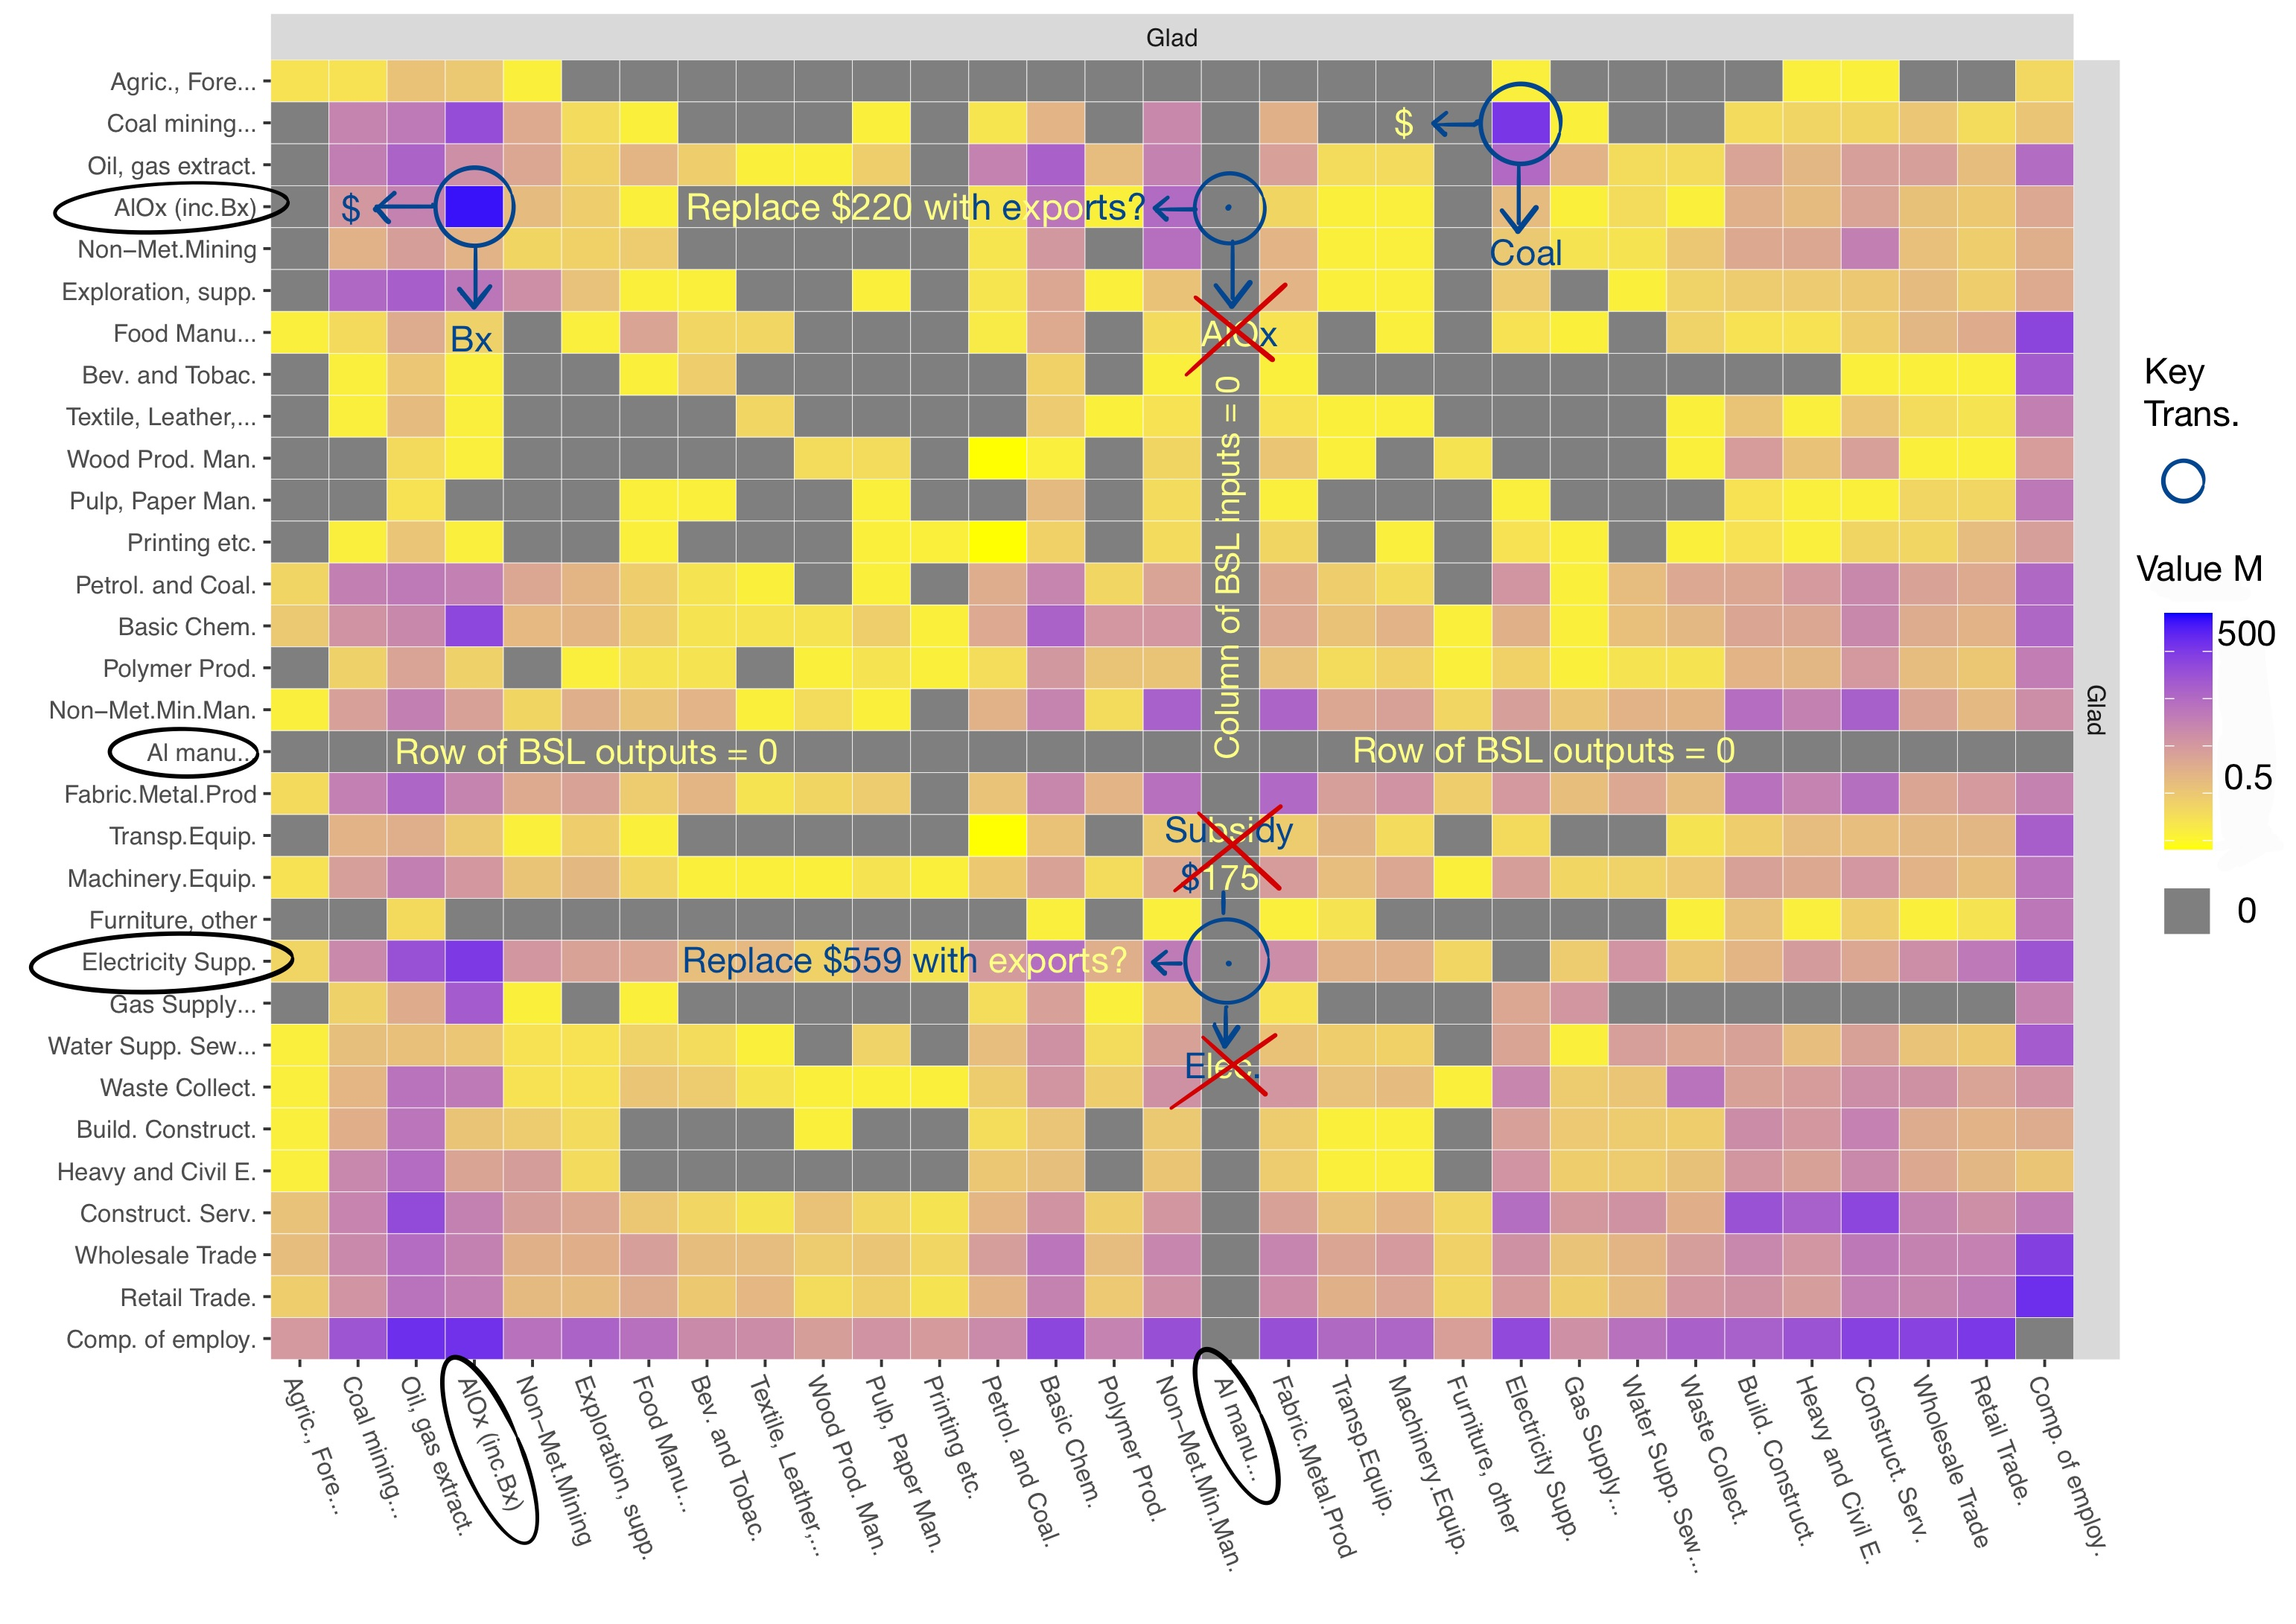
\includegraphics[width=0.98\textwidth]{./heatZvalexAl-ann.jpg}
  \end{figure}
 
  In all scenarios, we we impose a full extraction of BSL from the local economy
  and compare this to the status quo.  BSL is extracted from the economy by
  setting both the row and column associated with BSL in the transaction matrix
  $A$ to zero (see figure \ref{fig-exAl}). By setting the BSL row to zero, we
  are implicitly saying that all purchases of Al are now imported and therefore
  no longer part of the economy. By setting the BSL column to zero we are
  implicitly saying that BSL no longer purchases any goods or services from
  other sectors. The final step in the extraction is to set the final demand
  parameter of BSL to zero: this means that there are no exports of Al from
  Gladstone.

    In scenarios \eqref{AlEl-full}, \eqref{AlEl-par} and \eqref{AlEl-none}, the
  one-third extraction of Electricity Supply from the local economy is modelled as
  setting every transaction in the row and column associated with Electricity Supply to
  two thirds of the status quo value. This partial extraction reflects the fact
  that many aspects of the provision of electricity will continue to be supplied
  locally. For instance, maintainance of cables and measuring of meters will
  continue to take place after GPS is shut down. We choose to extract just one third
  of the Electricity Supply sector because that is a conservative estimate of
  the role of GPS and because it matches the  proportion of GPS employees to
  employment in the sector $\frac{1}{3} \approx 192 / 600$.  The fact that the exports are
  set to zero reflects the fact that Gladstone will no longer export power once
  GPS closes. Finally, the fact that, in scenario \ref{AlEl}, GPS purchases of coal are
  set to zero needs no explanation.

  
\subsection*{\centering Scenario Analysis of (exogenous) Exports}

Let us consider the possible responses that agents in the economy might have a
closure of BSL alone. As discussed above, it would seem reasonable for RT to
seek new buyers for the Alumina that BSL is no longer buying. These potential
buyers are necessarily outside of Gladstone (and indeed Queensland) and are
enter the model via exports. If RT were successful in fully replacing the
BSL\_AlOx purchase of \$209.6\textsc{m} with exports, then the revenues of
Gladstone’s AlOx refineries would not change and a significant part of the
upstream effects of a BSL closure would be mitigated.\footnote{We thank Brian
  Carrick and Liam Ramke for sharing their view that this would be a likely
  outcome during early discussions. }

  Now suppose that, in addition, for the scenario where GPS remains open and
  price movements in electricity and coal markets are such that it can maintain
  its current level of sales. Thereby fully replacing the BSL\_Electricity purchase
  of \$558.8\textsc{m} and, in effect, exporting this amount to rest of Queensland and the
  NEM. That is, GPS exports approximately $7,000\textsc{gwh} $ at wholesale
  prices of $\$80$ thereby replacing both BSL and the lost subsidy. In this
  case, which is captured by scenario \eqref{Al-full}, although the Gladstone
  economy has lost $\$744.5\textsc{m}$ in aluminium exports, the net decrease in
  Total Exports is
  \[ 209.6 + 558.8 - 744.5 = -\$24\textsc{m}.\] 
(A negative decrease is an increase.) This compensation via
  exports amounts to a significant \emph{automatic stabiliser} for the economy
  as we will see in the scenario analysis of GVA and employment below. In scenario \eqref{AlEl-full},
  where the BSL\_Electricity purchase is not replaced by exports, but where the GPS\_Coal purchase is, 
  total exports are 
  \[ 209.6 + 176.25 - 744.5 = \$359.6\textsc{m} \]

The percentage decreases in the following table are computed relative to status quo total exports of $\$7,279.6\textsc{m}$.

  % latex table generated in R 4.0.0 by xtable 1.8-4 package
% Tue Jun  2 04:19:39 2020
\begin{table}[H]
\centering
\caption{Decrease in Total Exports (\$\textsc{m}) per scenario} 
\begin{tabular}{lrrr|rrr}
  \hline
 &  (a) Full & (b) Part & (c) None & Full & Part & None \\ 
  \hline
(1) BSL & -24.0 & 110.8 & 757.0 & -0.3\% & 1.5\% & 10.4\% \\ 
  (2) BSL \& GPS & 359.6 & 391.4 & 758.0 & 4.9\% & 5.4\% & 10.4\% \\ 
   \hline
\end{tabular}
\end{table}


  For scenario \eqref{Al-par}, total exports decrease by \$110.8 relative to the
  status quo. This figure is
  calculated as follows:
  \[95\% \cdot 209.6 + 80\% \cdot 558.8 - 744.5 - 5\%\cdot 250,\] where
  $5\%\cdot 250 = \$ 12.5\textsc{m}$ represents the decrease in exports by
  downstream Fabrication of Aluminium Products, Transport Manufacturing,
  etc. due to the increased costs of importing Al from further afield. Clearly
  the main change relative to scenario \eqref{Al-full} is that GPS is only able
  to replace 80\% of the BSL\_Electricity transaction. Since the BSL\_El  purchase accounts for 75\% of 
  GPS output, in this scenario, we are modelling a fall of 15\% in
 total GPS  revenue. This fall is motivated by potentially lower prices that arise following the closure of BSL. 
 For scenario 
% \begin{remark}
%   Although a more thorough analysis of the elasticity of supply for GPS would be
%   required, we anticipate that the fact that GPS is a variable load power
%   station is important in this respect. Base-load power stations have a vertical
%   supply function and the inward shift in demand for electricity that arises due
%   to the closure of BSL results in a larger loss in revenues. In other words,
%   GPS would be able to reduce production and thereby reduce lost surplus.
% \end{remark}
  
  For scenario \eqref{Al-none}, the fall in exports is simple to calculate: the
  large fall of $\$744.5\textsc{m}$ in Al exports plus the downstream fall of
  $\$12.5\textsc{m}$. Although it is difficult to motivate the scenario where
  there is no response, it is worth bearing mind that this would be in keeping
  with a standard IO analysis. Moreover, it facilitates a comparison with
  scenario \eqref{AlEl-none}, where there is also no response and both BSL and GPS
  shut down: because the shock to final demand is similar.
  
  In all scenarios, the export multiplier is equal to 1 as exports are exogenously determined by external demand. This amounts to assuming that there are no indirect effects of the shock outside the local economy. This is a reasonable assumption given the fact that Gladstone-plus is small, and we are modelling the relevant upstream and downstream sectors endogenously (part of Gladstone-plus)


\subsection*{\centering Scenario Analysis of Gross Value Added}
We now present results for the endogenous measure of economic activity, GVA.  As per table \ref{tab-Glad-Aus}, the status quo level of total GVA is \$7625.5\textsc{m}. Percentage decreases in the following table are computed relative to the status quo. 

% latex table generated in R 4.0.0 by xtable 1.8-4 package
% Tue Jun  2 04:19:39 2020
\begin{table}[H]
\centering
\caption{Total Decrease in Gross Value Added (\$\textsc{m}) per scenario} 
\begin{tabular}{lrrr|rrr}
  \hline
 &  (a) Full & (b) Part & (c) None & Full & Part & None \\ 
  \hline
(1) BSL & 252.1 & 392.2 & 942.3 & 3.3\% & 5.1\% & 12.4\% \\ 
  (2) BSL \& GPS & 739.6 & 788.1 & 1121.3 & 9.7\% & 10.3\% & 14.7\% \\ 
   \hline
\end{tabular}
\end{table}

Even in the best scenario \eqref{Al-full}, GVA falls by  approximately \$250\textsc{m}. A substantial part of the difference between the central scenarios \eqref{Al-par} and \eqref{AlEl-par} is explained by the Electricity Sector (which has status quo Value Added of \$262.8):

% latex table generated in R 4.0.0 by xtable 1.8-4 package
% Tue Jun  2 04:19:39 2020
\begin{table}[H]
\centering
\caption{Total Decrease in Electricity Sector Value Added (\$\textsc{m}) per scenario} 
\begin{tabular}{lrrr|rrr}
  \hline
 &  (a) Full & (b) Part & (c) None & Full & Part & None \\ 
  \hline
(1) BSL & 1.1 & 35.1 & 173.9 & 0.4\% & 13.4\% & 66.2\% \\ 
  (2) BSL \& GPS & 221.1 & 221.3 & 223.8 & 84.1\% & 84.2\% & 85.2\% \\ 
   \hline
\end{tabular}
\end{table}

Note that the 84\% to 85\% loss in Electricity Sector Value Added in scenarios where GPS also closes is unsurprising given that  the BSL\_Electricity purchase represents 63\% of sector revenues. Indeed it is the loss of this and other transactions explains the higher GVA multiplier in scenarios \eqref{Al-none} and \eqref{AlEl-none} (see table \ref{tab-multgva}).\footnote{We define this multiplier as total (direct plus indirect) effect divided by the direct effect, where the direct effects on GVA are 
% latex table generated in R 4.0.0 by xtable 1.8-4 package
% Tue Jun  2 04:19:39 2020
\begin{table}[H]
\centering\footnotesize
\caption{\label{tab-chdgva}\footnotesize Direct Decrease in Gross Value Added (\$\textsc{m}) per scenario} 
\begin{tabular}{lrrr}
  \hline
 & Full & Part & None \\ 
  \hline
(1) BSL & 130.5 & 136.3 & 136.3 \\ 
  (2) BSL \& GPS & 218.1 & 223.9 & 223.9 \\ 
   \hline
\end{tabular}
\end{table}

}
% latex table generated in R 4.0.0 by xtable 1.8-4 package
% Tue Jun  2 04:19:39 2020
\begin{table}[H]
\centering
\caption{\label{tab-multgva}Gross Value Added multiplier per scenario} 
\begin{tabular}{lrrr}
  \hline
 & Full & Part & None \\ 
  \hline
(1) BSL & 1.9 & 2.9 & 6.9 \\ 
  (2) BSL \& GPS & 3.4 & 3.5 & 5.0 \\ 
   \hline
\end{tabular}
\end{table}



In the present paper, the subsidy is run through the Aluminium Manufacturing sector. If instead we were to run the subsidy through the Electricity Sector, although the aggregate effects would be similar, we would see an increase Value added for the Electricity Sector in scenarios \eqref{Al-full}--\eqref{Al-none}. For expositional purposes, we present the result for that treatment of the subsidy in figure \ref{fig-sub-el}.

\begin{figure}
\includegraphics[width=.98\textwidth]{./GVA2fine.jpg}
\caption{\label{fig-sub-el} In this figure, for our central scenarios \eqref{Al-par} and \eqref{AlEl-par}, the subsidy instead runs through the Electricity Sector. In scenario \eqref{Al-par}, Electricity Sector Value Added increases (the downward spike). We also see small increases in VA in other sectors due to the public sector multiplier. We  observe similar effects following the closure of the Kurri Kurri and Point Henry smelters. }
\end{figure}



\subsection*{\centering Scenario analysis of aggregate employment}
Recall that there are 920 employees at BSL and 192 employees at GPS. Following
consultation with QTC, we model these jobs as premium, with average (mean)
annual employee compensation of just over $\$117\textsc{k}$ (including
superannuation).  The average annual compensation for the rest of the broader
Gladstone economy is taken to be $\$107\textsc{k}$.\footnote{According to
  Regional Profiles Data, the ratio of the median worker in Gladstone to the
  median worker in QLD is $1.213$. The average (mean) employee compensation
  (including superannuation) for QLD is very close to
  $\$107\textsc{k}/ 1.213 \approx \$88\textsc{k}$. }

For our broader definition of Gladstone, with
an \emph{effective workforce} of $31,694$, we obtain the following
table of direct job losses.   

% latex table generated in R 4.0.0 by xtable 1.8-4 package
% Tue Jun  2 04:19:39 2020
\begin{table}[H]
\centering
\caption{\label{comjldex} Direct decrease in employment (\textsc{fte}) per scenario} 
\begin{tabular}{lrrr|rrr}
  \hline
 &  (a) Full & (b) Part & (c) None & Full & Part & None \\ 
  \hline
(1) BSL & 920 & 955 & 955 & 2.9\% & 3.0\% & 3.0\% \\ 
  (2) BSL \& GPS & 1112 & 1147 & 1147 & 3.5\% & 3.6\% & 3.6\% \\ 
   \hline
\end{tabular}
\end{table}

  
Table \ref{comjldex} confirms that in scenario \eqref{Al-full} the only job
losses those in the employment of BSL. In \eqref{AlEl-full}, the figure
$1,112 = 920 + 192 $ is the sum of the losses at BSL and GPS. In the other four
scenarios, the additional $35$ job losses are coming from the downstream sectors
(Fabrication of Metal Products, Transport and Equipment Manufacturing and
 Machinery Manufacturing). This minor effect is the result of our $5\%$
extraction of these sectors to capture the impact of a small but significant rise in the
local price of aluminium. We argue that this is plausible given that these
sectors will have to source their purchases from further afield in absence of
BSL.
  
% latex table generated in R 4.0.0 by xtable 1.8-4 package
% Tue Jun  2 04:19:39 2020
\begin{table}[H]
\centering
\caption{\label{comjlinex} Indirect decrease in employment (\textsc{fte})  per scenario} 
\begin{tabular}{lrrr|rrr}
  \hline
 &  (a) Full & (b) Part & (c) None & Full & Part & None \\ 
  \hline
(1) BSL & 356 & 927 & 3120 & 1.1\% & 2.9\% & 9.9\% \\ 
  (2) BSL \& GPS & 2190 & 2392 & 3570 & 6.9\% & 7.6\% & 11.3\% \\ 
   \hline
\end{tabular}
\end{table}

 
Table \ref{comjlinex} shows that the extent to which exports respond is
vital in explaining indirect effects. In scenario \eqref{Al-full}, exports of AlOx and Electricity fully
compensate and as a consequence, the indirect job losses are less than half of direct losses.
In scenario \eqref{AlEl-full}, although exports compensate for
the BSL\_AlOx transaction and the GPS\_Coal transaction, the absence of GPS
means that the economy suffers a total loss of the BSL\_Electricity
transaction. As a consequence, indirect job losses are almost twice direct losses.
 
In our central subscenarios, a similar, but less stark conclusion holds. In
scenario \eqref{Al-par}, where exports compensate for $95\%$ of the BSL\_AlOx
transaction and $80\%$ of the BSL\_Electricity transaction, indirect 
job losses are just similar to direct losses.  In scenario
\eqref{AlEl-par}, where exports compensate for $95\%$ of both the BSL\_AlOx and
the GPS\_Coal transactions, but the BSL\_Electricity transaction is lost,
indirect job losses are more than twice direct losses.

Finally, in the worst case, where exports do not compensate at all, we see that
indirect job losses are rather similar: the ratios of indirect to direct job
losses are both above $3$ and in fact higher in scenario \eqref{Al-none} than in
\eqref{AlEl-none}.

These ratios are also reflected in the following employment multipliers.
 
% latex table generated in R 4.0.0 by xtable 1.8-4 package
% Tue Jun  2 04:19:39 2020
\begin{table}[H]
\centering
\caption{\label{multchwex}Total Employment (\textsc{fte})  multiplier per scenario} 
\begin{tabular}{lrrr}
  \hline
 & Full & Part & None \\ 
  \hline
(1) BSL & 1.4 & 1.9 & 4.0 \\ 
  (2) BSL \& GPS & 2.8 & 2.9 & 3.8 \\ 
   \hline
\end{tabular}
\end{table}


 
We conclude the analysis of aggregate employment for the Gladstone economy with
the total (direct plus indirect) impact on employment.

% latex table generated in R 4.0.0 by xtable 1.8-4 package
% Tue Jun  2 04:19:39 2020
\begin{table}[H]
\centering
\caption{\label{comjltotex}Total decrease in employment (\textsc{fte})  per scenario} 
\begin{tabular}{lrrr|rrr}
  \hline
 &  (a) Full & (b) Part & (c) None & Full & Part & None \\ 
  \hline
(1) BSL & 1276 & 1882 & 4075 & 4.0\% & 6.0\% & 12.9\% \\ 
  (2) BSL \& GPS & 3302 & 3539 & 4717 & 10.4\% & 11.2\% & 14.9\% \\ 
   \hline
\end{tabular}
\end{table}


% In scenario
% \eqref{Al-none}, indirect losses are almost $3\frac{1}{2}$ direct losses. In
% \eqref{AlEl-none}, indirect losses are just over $3\frac{1}{8}$ of direct losses.
\label{sec-emp-agg}
\subsection*{\centering Analysis of employment by sector}
\label{sec-emp-sectoral}

In section \ref{sec-emp-agg}, we showed that the indirect effects on aggregate
employment for the combined closure of BSL and GPS. One reason for this
relatively large indirect effect is that, Employee Compensation for Electricity
Supply in scenario \eqref{Al-full} is essentially the same as the status
quo. This implies no job losses to the sector in that scenario with employment
at approximately $600$.  In scenario \eqref{AlEl-full}, employment in
Electricity Supply falls to around $100$. Given the basic inelasticity of demand for electricity and the services
associated with the delivery of electricity such as cable mainenance and
electricians, it seems unlikely that employment in Electricity Supply would
indeed to fall to such a low level. The overshooting of the model is an artifact
of the linearity of the present model and its inability to capture inelastic
demand for electricity.  One solution would be to run a nonlinear version of the
present model, but due to time constraints this is beyond the scope of the
current modelling exercise. Instead, we  reallocate job losses from Electricity Supply to
other sectors that remain open on a pro rata basis (depending on its original
level of employment). Since there are 68 other sectors, the change for each
sector relative to its original size is negligible. This ensures that, in all
scenarios, job losses to Electricity Supply are no higher than half the total
for the sector.  Figure \ref{jl-lolly} shows that there are approximately $300$
job losses to Electricity Supply in every scenario except \eqref{Al-full} and
\eqref{Al-par}. It also highlights the other sectors that are likely to suffer
large job losses.
 
      
\begin{figure}[H]
  \caption{\label{jl-lolly}Total job losses across all 70 sectors and all six  scenarios. The two main losses are to the smelter and the power station. In scenario \eqref{Al-full}, there are no losses to Electricity Supply, AlOx, Coal Mining or Fabrication of Metal Products.}
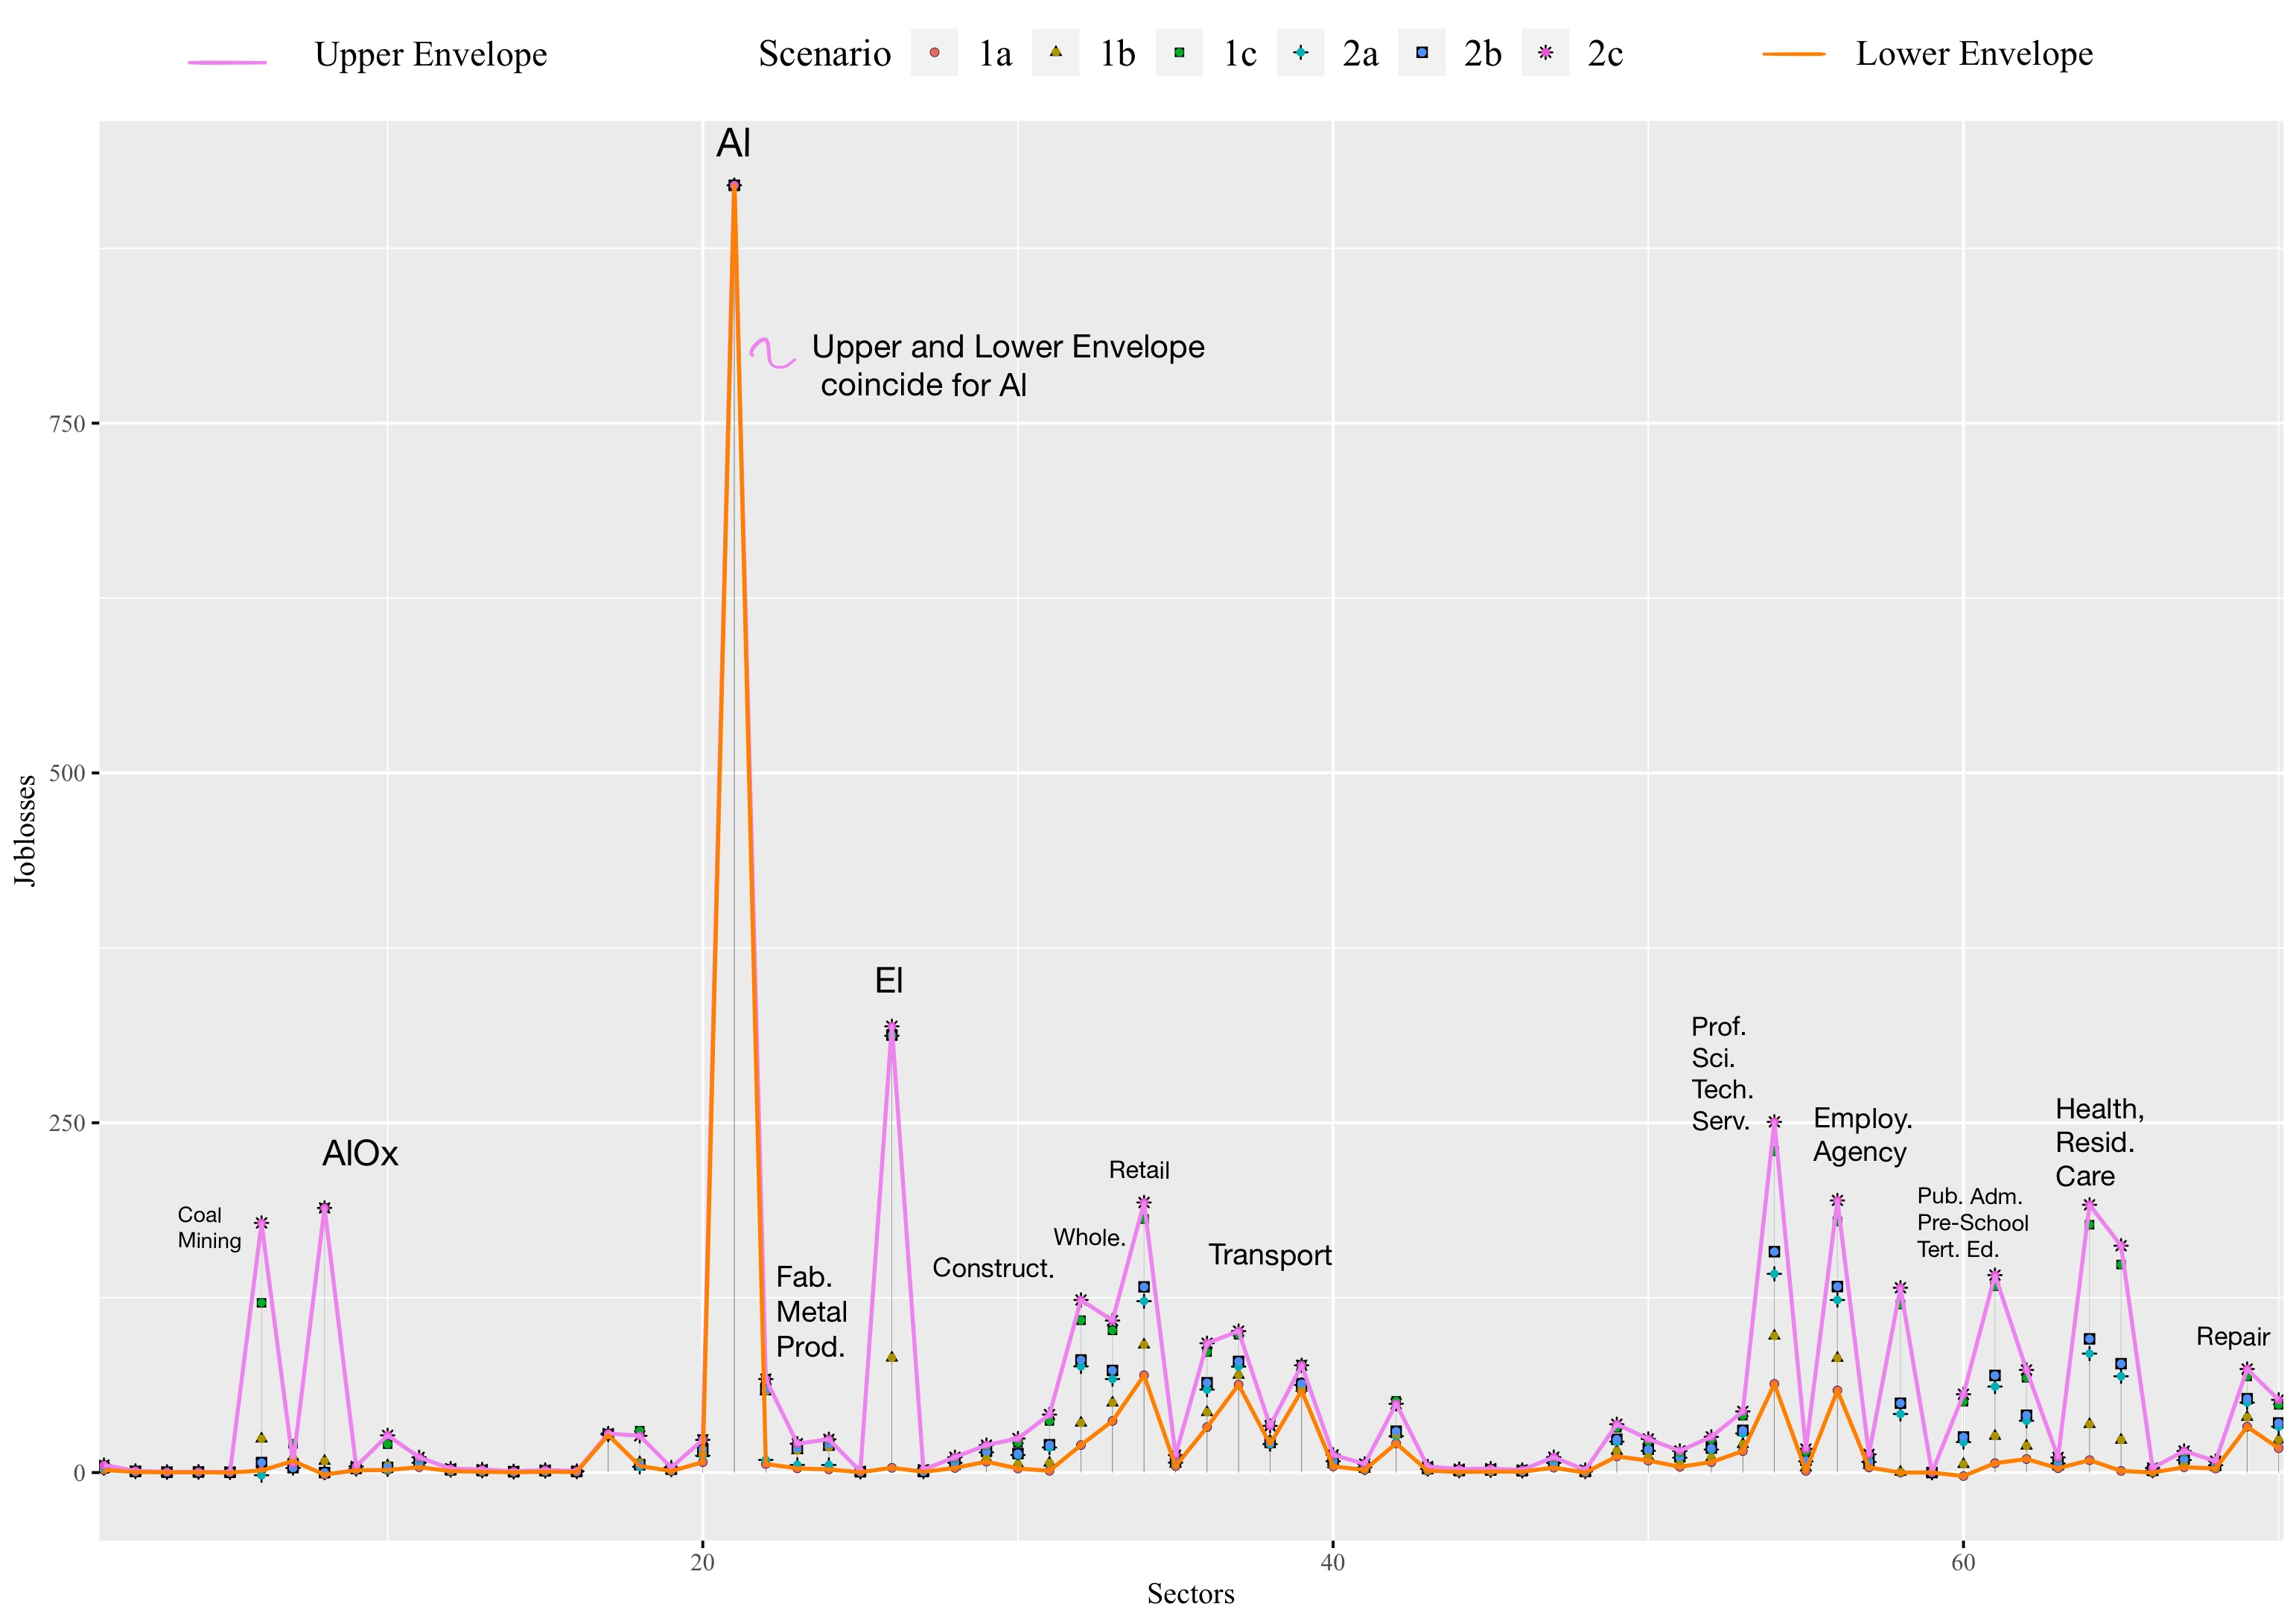
\includegraphics[width=.98\textwidth]{./jl-lolly-annotated.jpg}
\end{figure}

For scenario \eqref{AlEl-full}, beyond Aluminium production and Electricity
Supply, indirect job losses in other sectors number 500 in total.  The sector
with the next highest number of job losses is sector $54$ (Professional,
Scientific and Technical services) is the sector with the next highest job
losses at $198$. Beyond this, sector $56$ (Employment, Travel Agency and Other
Administrative Services) sees job losses of $130$ and sector $34$ (Retail) a
further $111$ job losses.

As figure \ref{jl-lolly} shows, the job losses in these sectors increase further
in scenarios \ref{Al-none} and \ref{AlEl-none}, where exports do not
compensate for the loss of the other key transactions (BSL purchases of AlOx and
GPS purchases of Coal). (The impact of these two transactions is visible as
smaller spikes to the left of the figure.)



 
\section*{\centering Conclusions}
In our view, BSL purchases of AlOx are likely to be replaced by exports in the
event of a shut down. High elasticity of demand in international markets would
ensure that the upstream producers of Bx and Alumina would recover quickly.  In
the short run at least, given the volume of coal that passes through Gladstone
port, GPS purchases of (thermal) Coal would also recover quickly. In other
words, scenarios \eqref{Al-none} and \eqref{AlEl-none} are unlikely to
materialise.

It is less obvious that GPS “exports” would replace BSL purchases of Electricity
in the event that it remained open. Support for the idea that GPS would comes
from the observation that GPS currently competes with other participants to sell
its electricity to the grid. On the other hand, the fact that GPS is currently
operating below capacity (at around 60\%) is a consequence of inefficiencies
associated with the age of the power station. But it also reflects subsidies to
other, cleaner forms of energy. It is important to note that, in the present
setting, the subsidy that CS Energy provides to BSL, is indirect. If BSL were to
close, the likely fall in electricity prices would render GPS less
competitive. 
\begin{itemize}
\item The central scenarios capture what we view as the
most plausible outcomes. 
\end{itemize}

Given that GPS is a variable load power station with
significant capacity provides the East Coast electricity market with insurance (a put option) against volatile
 electricity prices and potential blackouts. Indeed, assuming
that BSL were to shut down, this option value suggests that there may be a
smaller subsidy that might be worthwhile to keep GPS open at least until a
genuine replacement source of power is established. If for clean energy reasons, a coal-fired power station in Queensland is to shut down, it is worth considering other power stations as the opportunity cost of closing GPS is high.  Even if the economic impact of a GSP closure on Gladstone itself (as opposed to Gladstone-plus) is less smaller than the impact we identify here, it is bound amplify the impact of the closure of BSL. Closing a coal-fired power station in a different region of Queensland might help to spread the burden across a wider geographical area.

What we do not measure in this study is the benefit to consumers  of a fall in
electricity prices that would follow the shut down of BSL. A more complete social welfare
analysis would entail measurement of the likely movement in electricity prices,
something that is beyond the scope of the present study.

Planning is the key to transition and a successful transition would make all the
difference in event that BSL and, eventually, GPS close. The Kurri Kurri smelter
in NSW is still in early stages of decommissioning and the local Hunter Region community is 
still in the process of planning \emph{8 years} after the smelter initially
closed down. Although aggregate employment has almost-fully recovered, the
manufacturing sector for the Hunter Region is significantly smaller than it was
in 2011. 

\begin{thebibliography}{1}


\bibitem{Dann} Queensland Treasury Corporation (Peter Dann), “Boyne Island
  Smelter: Economic impact on the Gladstone Region and Queensland,” 2019

\bibitem{Brook}
Queensland Treasury Corporation (Peter Brook), “Aluminium in QLD: Rio Tinto,” 2019
  
\bibitem{subsidies}
C. Hamilton and H. Turton, ``Subsidies to the Aluminium
Industry and Climate Change,'' The Australia Institute, 1999, https://www.tai.org.au/sites/default/files/WP21\_8.pdf

\bibitem{abs} Australian Bureau of Statistics (ABS), “2016-2017 Table 5: Industry by
  Industry Flow Table (Direct Allocation of Imports),” released at 11.30am
  (Canberra time) 19 July 2019, https://www.abs.gov.au/AUSSTATS/abs@.nsf/DetailsPage/5209.0.55.0012016-17?OpenDocument

\bibitem{port}
 Port of Gladstone, ``Trade Statistics Data,''
 https://www.gpcl.com.au/trade-statistics, Retrieved  April 26 2020

\bibitem{RT}
  Rio Tinto, ``Annual Report: Production, Reserves and Operations,''
https://www.riotinto.com/invest/reports/annual-report, 2019, Retrieved on
27 April 2020

\bibitem{reg-prof}
  Queensland Government Statistician’s Office,
  “Queensland Regional Profiles,”
https://statistics.qgso.qld.gov.au/qld-regional-profiles, Retrieved 26 April 2020 
 
\bibitem{id-comm}
  .idcommunity, “Regional resources,” 
  https:// economy.id.com.au/gladstone, Retrieved 27 April 2020

  \bibitem{manu-lab-share}
B. Berger and G. Wolff, “The global decline in the labour income share: is
capital the answer to Gernmany’s current account surplus?,” Policy Contribution,
Issue 12, April 2017

\bibitem{GPS-2029} Energy Matters, “Gladstone Power Station: We will operate
  beyond 2029,”
  https://www.energymatters.com.au/renewable-news/gladstone-power-station-remain-open-2029/,
  8 August 2018

\bibitem{AEMO}
  Australian Energy Market Operator, “Draft 2020 Integrated System Plan,”
  https://aemo.com.au/energy-systems/major-publications/integrated-system-plan-isp/2020-integrated-system-plan-isp,
  12 December 2019

\bibitem{bat}
  G. Cusano, M. R. Gonzalo, F. Farrell, R. Remus, S. Roudier, L. Delgado Sancho,   “Best Available Techniques (BAT) Reference Document for the
  Non-Ferrous Metals Industries,” EUR 28648, doi:10.2760/8224, 2017

\bibitem{CSE}  
  CS Energy, ``Statement of Corporate intent," 2015/2016
  
%G. Eason, B. Noble, and I. N. Sneddon, ``,'' Phil. Trans. Roy. Soc. London,
%vol. A247, pp. 529--551, April 1955.

  

\end{thebibliography}


\end{document}



%%% Local Variables:
%%% mode: latex
%%% TeX-master: t
%%% End:

